\documentclass[8pt]{article}

\usepackage[utf8]{inputenc}
\usepackage[ngerman]{babel}
\usepackage{amsmath}
\usepackage{nicefrac}
\usepackage{color}
\usepackage[hidelinks]{hyperref}
\usepackage{graphicx}
\usepackage{stmaryrd}
\usepackage[a4paper,top=2cm,left=4cm,right=4cm,bottom=2cm,marginparwidth=5cm]{geometry}
\usepackage{marginnote}
\usepackage[automark]{scrpage2}
\pagestyle{scrheadings}

\newcommand{\fatnote}[1]{\marginnote{\textbf{#1}}}
\newcommand{\leftnote}[1]{\reversemarginpar\fatnote{#1}}
\newcommand{\rightnote}[1]{\normalmarginpar\fatnote{#1}}

\newcommand{\defin}[1]{\noindent #1\vspace{0.3cm}}
\newcommand{\ldefin}[2]{\leftnote{#1}\defin{#2}}
\newcommand{\rdefin}[2]{\rightnote{#1}\defin{#2}}

\newcommand{\todo}[1]{\textcolor{red}{\textbf{TODO}: #1}}

\newcommand{\coursename}{\@empty}
\newcommand{\groupno}{\@empty}

\newcommand{\course}[2]{\renewcommand{\coursename}{#1}\renewcommand{\groupno}{#2}}
\newcommand{\beginsheet}{\clearscrheadfoot\ihead[]{Kurs: \coursename}\ohead[]{Gruppe \groupno}\ofoot[]{\pagemark}\ifoot[]{Dieses Dokument ist Teil der Dokumentation}}

\newcommand{\email}[1]{\href{mailto:#1}{#1}}


%%%%%%%%%%%%%%%%%%%%%%%%%%%%%%%%%%%%%%%%%%%%%%%%%%%%%%%%%%%%%%%%%%%%%%%%%%%%%%%%%%%%%%
%% Oberhalb dieses Blocks nichts ändern
%%%%%%%%%%%%%%%%%%%%%%%%%%%%%%%%%%%%%%%%%%%%%%%%%%%%%%%%%%%%%%%%%%%%%%%%%%%%%%%%%%%%%%


%% TODO: Hier die fehlende Gruppennummer einfügen
\course{Lisp Kurs -- Roboterprogrammierung in Lisp}{4}


\begin{document}

\beginsheet

\title{SUTURObot}
\author{Jannik Buckelo, Simon Stelter}
\date{13.07.2014}
\maketitle

\newpage

\tableofcontents

\newpage

\begin{abstract}
Dokumentation des SUTURObots der im Rahmen des Lisp Tutorials an der Universit"at Bremen erstellt wurde. Zur Konstruktion des Roboters wurde ein LEGO Mindstorm verwendet, der mittels eines Smartphones gesteurt werden kann. Die Steuerung der Motoren und das Auswerten der Sensoren wird dabei von einem Common Lisp-Programm geregelt.	
\end{abstract}

\section{einleitung} simon\\
Im Rahmen eines Lisp Tutorials haben wir mit LEGO Mindstorm Roboter gebaut und dann mit Lisp gesteuert. Es wurde als erstes der SUTURObot v1 \ref{fig:SUTURObot1} gebaut, dieser sollte auf zwei parallel ausgerichteten Rädern stehen können. Für die Bestimmung der Lage sollte ein Smartphone verwendet werden, welches mit einer Android-App die Lage des Handy's ausliest und an das Lisp programm zur verarbeitung sendet.\\
Da dieser selbst gebaut Sensor für das Vorhaben jedoch zu langsam war, wurde der SUTURObot v2 \ref{fig:SUTURObot2} entwickelt. Dieser hat eine holonome Basis und soll mit der vorher entwickelten Android-App frei bewegt werden können. Zusätzlich sollte er auf Kollisionen reagieren können.

\section{SUTURObot v1}
\begin{figure}[h]
  \begin{center}
    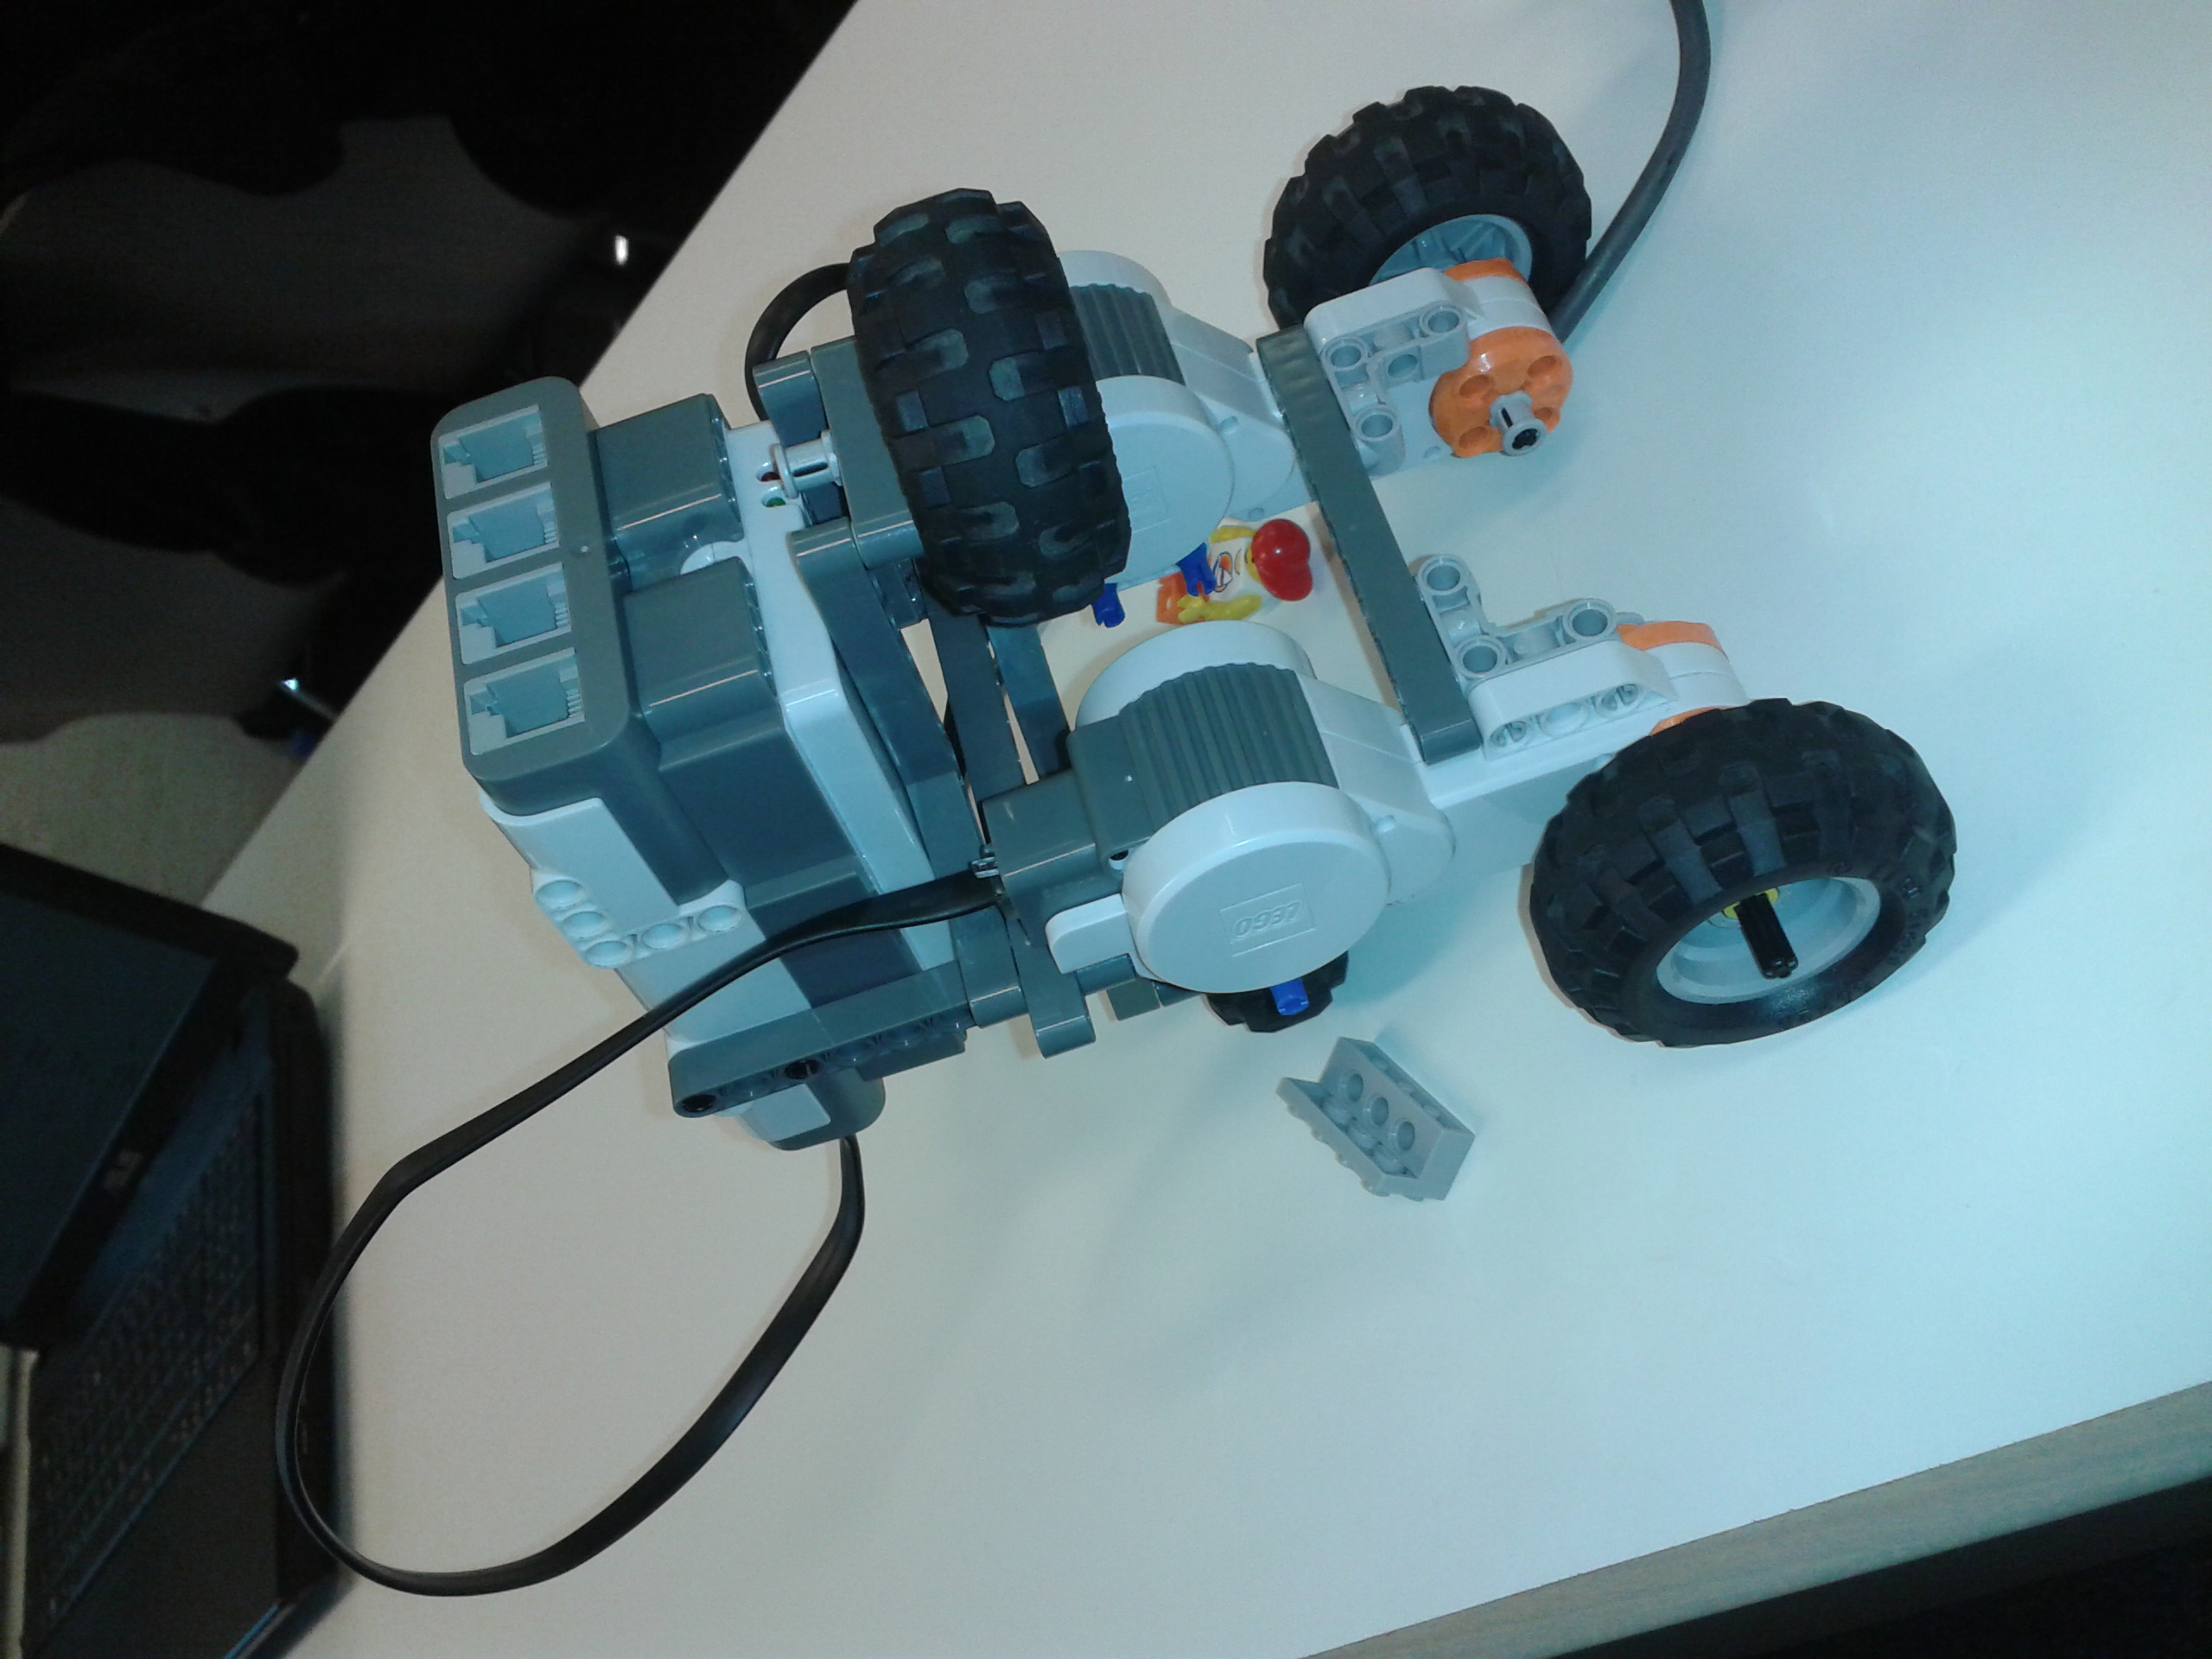
\includegraphics[width=.5\textwidth]{pictures/SUTURObot-v1.jpg}  
  \end{center}
  \caption{SUTURObot v1}
  \label{fig:SUTURObot1}
\end{figure}

\subsection{Idee und Lösungsansatz} simon
Wir haben uns am Anfang dafür entschieden einen Roboter zu bauen, der auf zwei parallel stehenden Rädern balancieren und fahren kann. Dafür benötigten wir passende Sensor, um die Lage des Roboters zu bestimmen. Da uns kein Gyrosensor von Lego zu Verfügung stand und die Daten aus dem Ultraschallsensor zu stark mit Rauschen belastet waren, haben wir uns dafür entscheiden, den Lagesensor eines Smartphones zu verwenden. Unsere grundlegende Idee war es dann aus der Lage den Fehler zu bestimmen und mit einem PID-Controller die Balance zu halten bzw zu fahren. Von Balancieren sollte zum Fahren gewechselt werden, indem mittels des PID-Controllers eine leicht gekippte Haltung eingenommen wird.

\subsection{architektur}

\subsubsection{allgemein} jannik

\subsubsection{Sensorik} 
simon\\
Um den Lagesensor des Smartphones auszulesen haben wir eine Android-App geschrieben, die den ausgelesenen Quaternion unverändert auf einem topic veröffentlicht.
Für unser Vorhaben war es nötig aus dem Quaternion die Neigung zu bestimmen. Dazu reichte jedoch keine einfache Umrechnung in Eulerwinkel, da zum einen die Lösung nicht eindeutig ist und zum anderen es unter bestimmten Bedingungen überhaupt keine gibt. Wir haben daher die Funktion \texttt{pitch} implementiert um die Neigung zu berechnen. In dieser erstellen wir zwei identische Vektoren, $\left( \begin{array}{c} 1 \\ 0 \\ 0
\end{array} \right)$. Einen davon rotieren wir mit der Quaternion vom Handy. Wenn wir nun den Winkel zwischen beiden bestimmen, erhalten wir die Neigung. Da jedoch mit diesem Verfahren sowohl eine Vorwärts-, als auch eine Rückwärtsneigung einen positiven Winkel liefert, neigen wir den zweiten Vektor vor der Winkelbestimmung um $pi / 2$. Wenn wir dann von der gewonnenen Neigung $pi / 2$ abziehen, kann man zwischen einer Vorwärts- und Rückwärtsneigung anhand des Vorzeichens unterscheiden.

\subsection{Probleme} simon\\
Tests mit dem SUTURObot v1 haben ergeben, dass der Lagesensor das Handy selbst, oder auch die Datenübertragung zu viel Zeit in Anspruch nimmt, um mit den Motoren einem Stürz rechtzeitig entgegen wirken zu können. Da uns leider kein weiteres Handy mit den passenden Sensoren zu Verfügung stand, um den die erste Fehlerquelle auszuschließen, haben wir uns schweren Herzens dafür entschlossen, stattdessen den SUTURObot v2 zu entwickeln.

\section{SUTURObot v2}
\begin{figure}[h]
  \begin{center}
    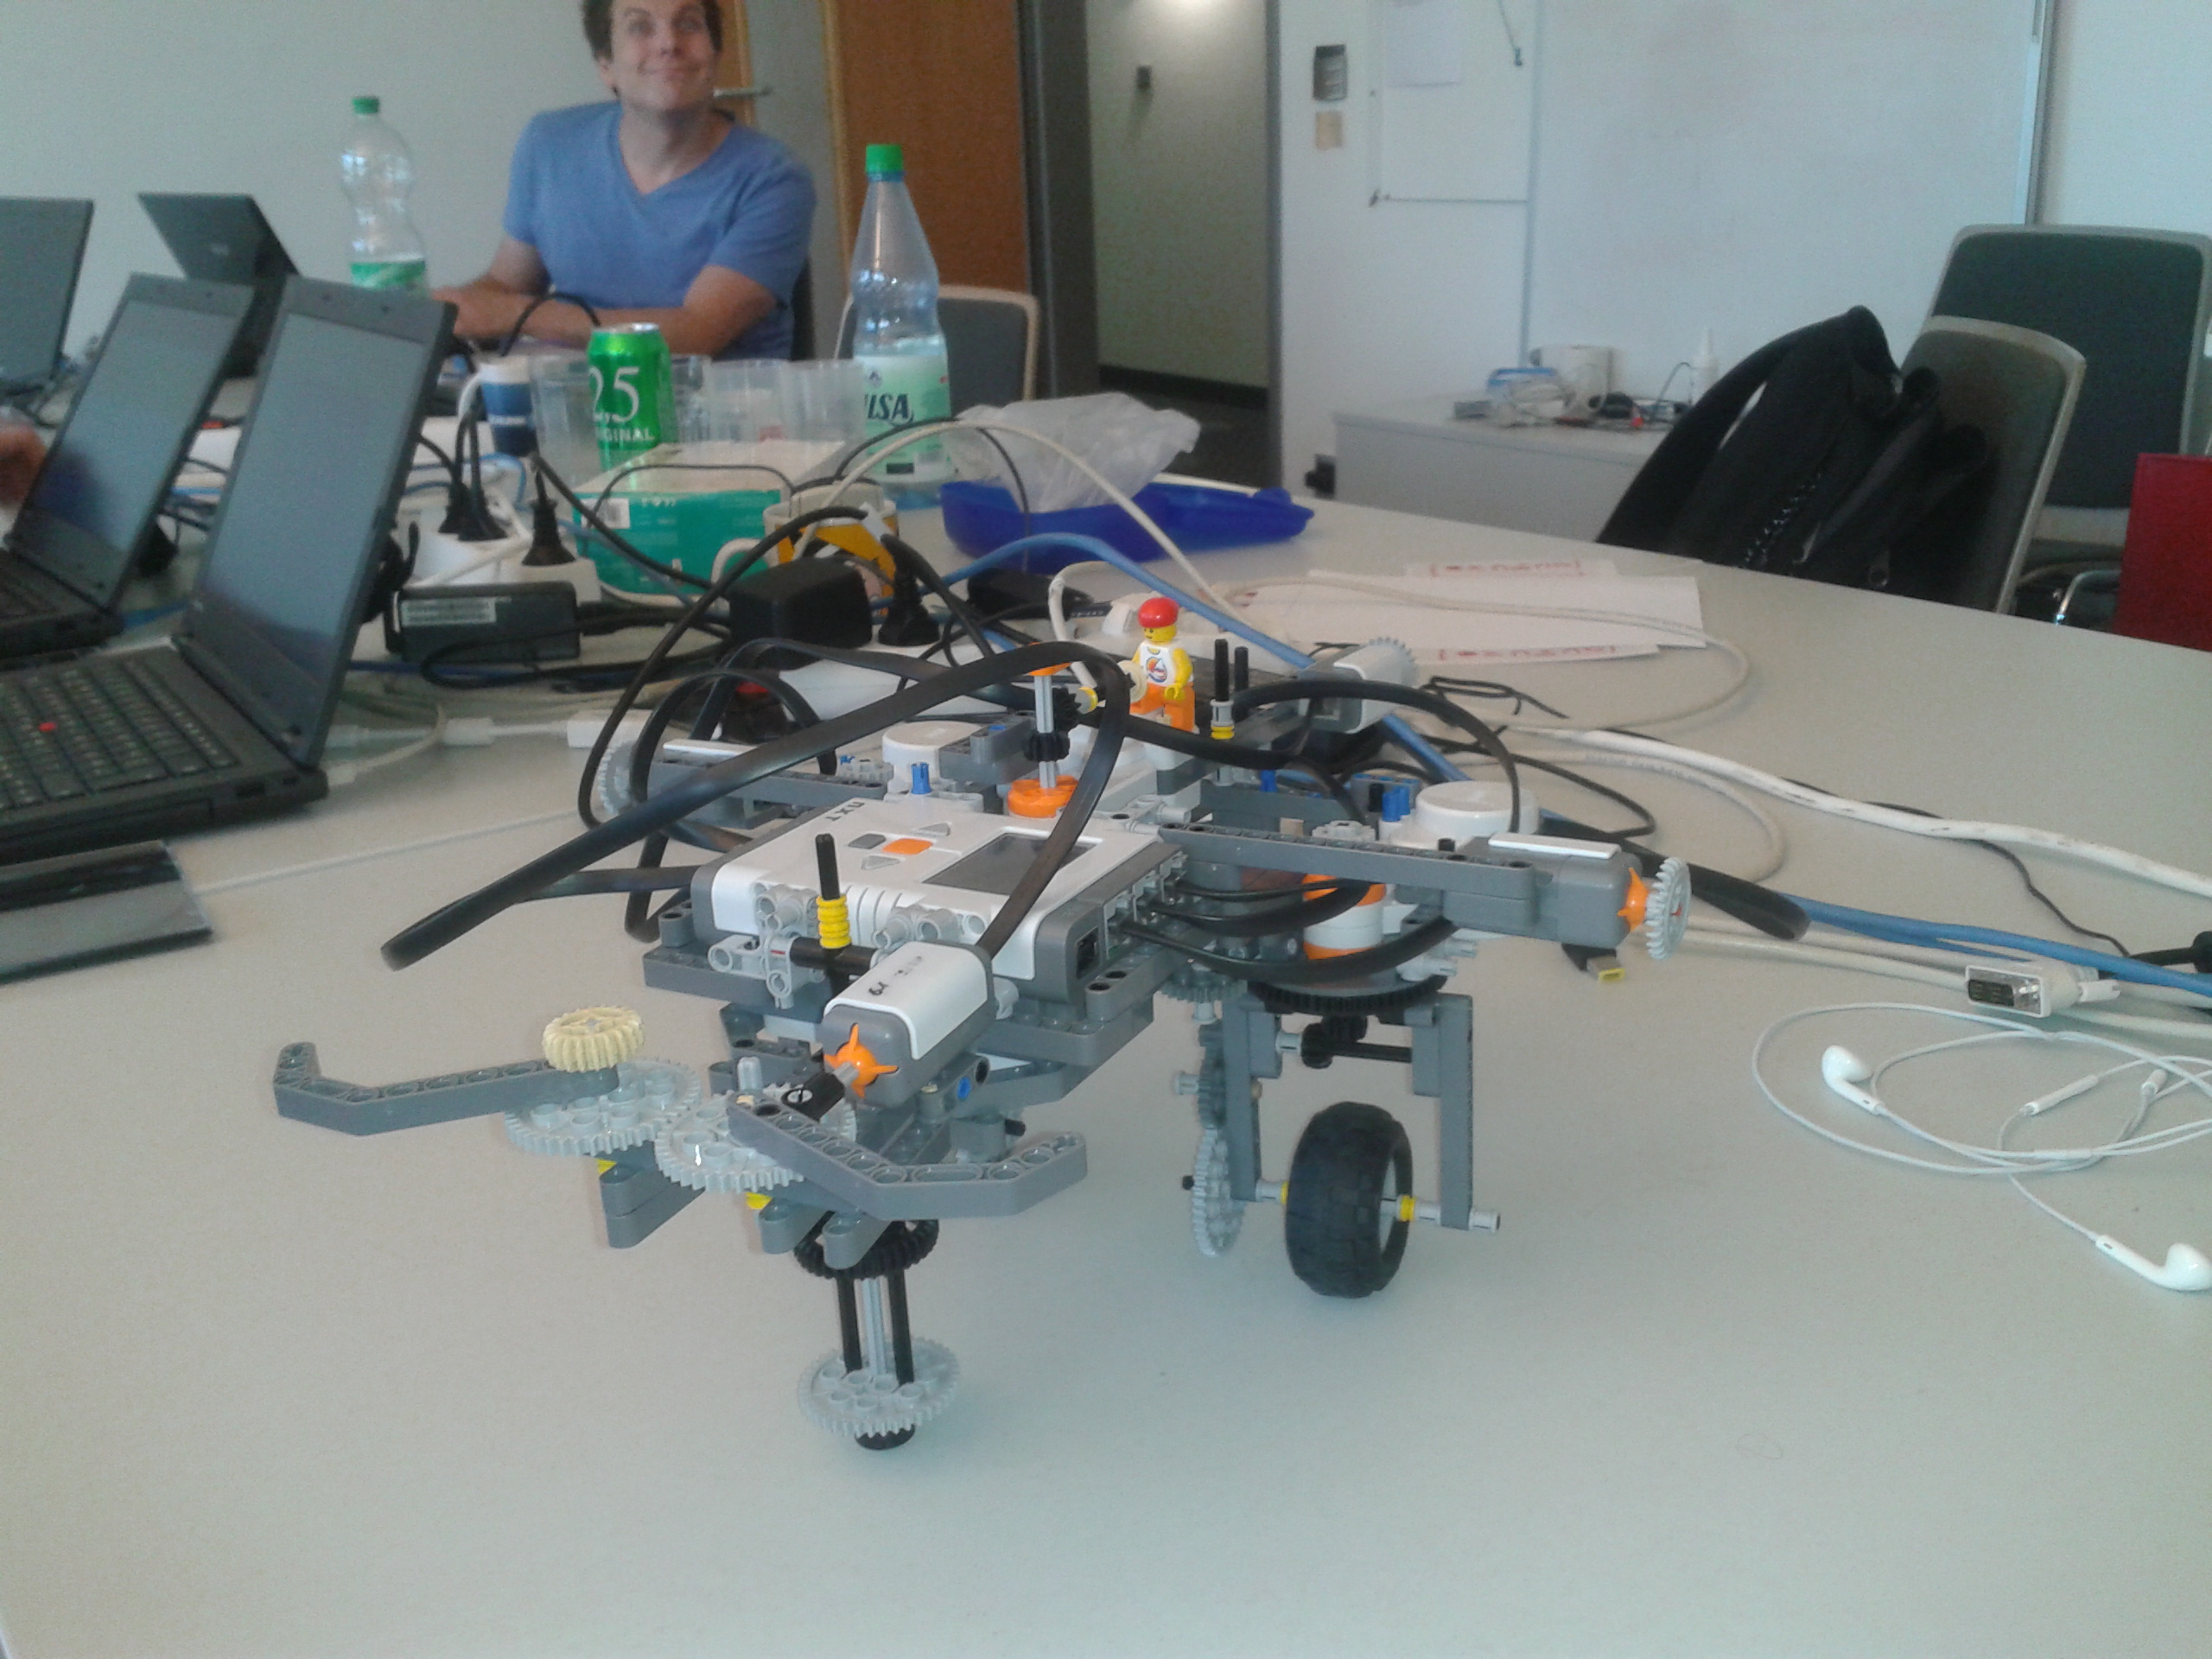
\includegraphics[width=.5\textwidth]{pictures/SUTURObot-v2.jpg}
  \end{center}
  \caption{SUTURObot v2}
  \label{fig:SUTURObot2}
\end{figure}

\subsection{lösungsansatz + idee} jannik
Nachdem unser SUTURObot v1 aus vorher beschriebenen Gr"unden nicht funktionert hat, mussten wir uns ein neues Konzept ausdenken. Wir wollten dabei m"oglichst viel von unserem bis dahin erstellten Code und Infrastruktur wiederverwenden. Also haben wir uns "uberlegt die bereits bestehende Android-App und Funktionen zur Lagebestimmung des Handys zu verwenden, um den Roboter zu steuern.

Wir haben dazu eine holonome Basis f"ur den Roboter gebaut und die App mit zwei zus"atzlichen Buttons ausgestattet, sodass der Effort der R"ader mittels kippen des Smartphones geregelt werden kann und die Drehung der R"ader mittels Buttonklick. Au"serdem haben wir vier Drucksensoren an den Seiten des Roboters zur Erkennung von Kollisionen angebracht. Sollte es zu einer Kollision kommen soll der Roboter selbst"andig die Bewegung in Richtung des Hindernisses einstellen und ein St"uck von dem Hindernis wegfahren.

\subsection{architektur}
top down

\subsubsection{allgemein} jannik



\subsubsection{sensorik} jannik


Wie schon erwähnt verwenden wir unter anderem wieder das Smartphone um

\subsubsection{Visualisierung} simon\\
Für Debugging Zwecke haben die Datei \texttt{marker.lisp} erstellt, diese enthält Funktionen um die vom Handy empfangenen Daten in Rviz zu visualisieren. Mit den Funktion \texttt{effort-visualization} und \texttt{rudder-effort-visualization} lassen sich die Motorkommandos anzeigen und mit \texttt{visu-handy} wird eine blaue Box verwendet um die Lange des Handys in Rviz darzustellen.
\begin{figure}[h]
  \begin{center}
    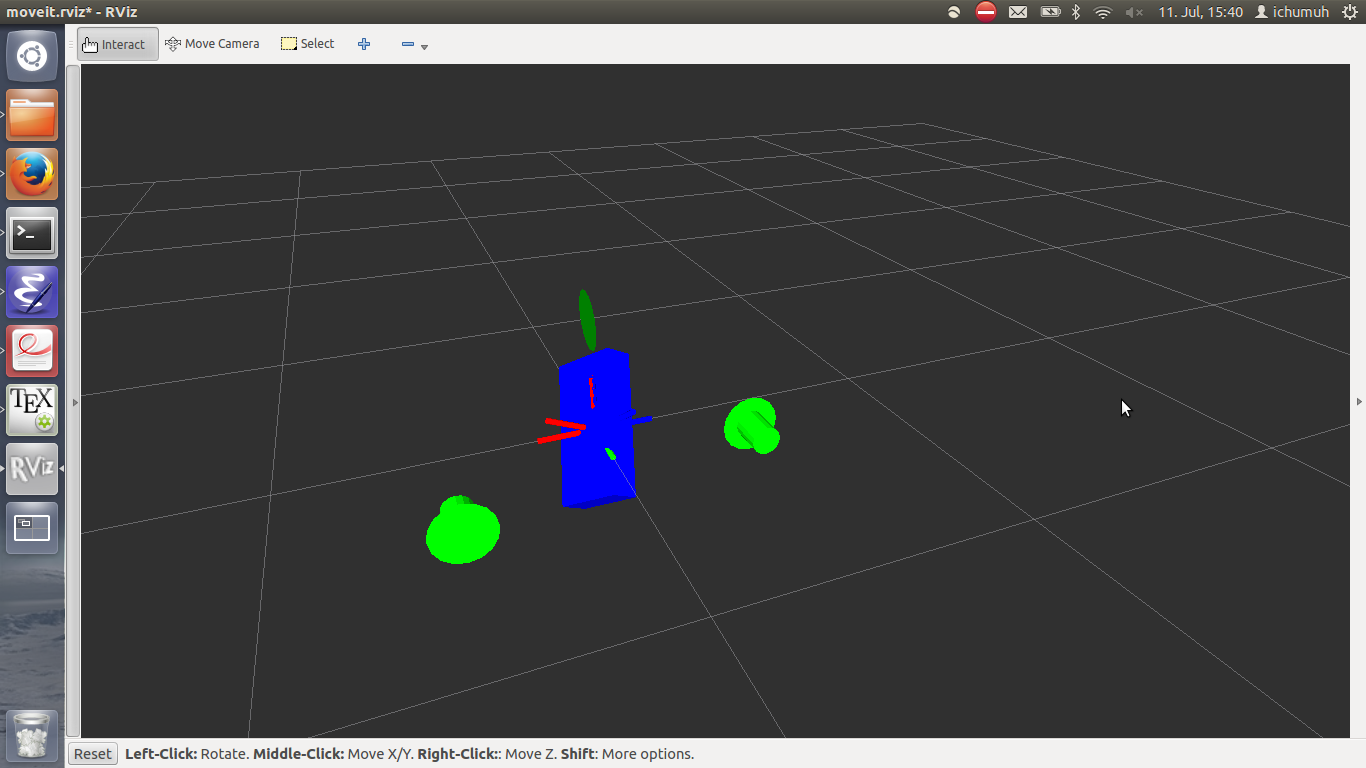
\includegraphics[width=.4\textwidth]{pictures/rviz2.png}
    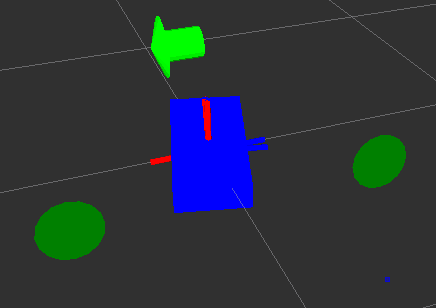
\includegraphics[width=.5\textwidth]{pictures/rviz1.png}    
  \end{center}
  \caption{Darstellung der Handydaten und Motorkommandos in Rviz}
  \label{fig:pancake}
\end{figure}

%\includegraphics[scale=1]{asd}

\subsection{Probleme} simon

Wir hatten während der Konstruktion mit der 

\end{document}








